%&"../main"
\documentclass[../main]{subfiles}
\begin{document}

\chapter{通用DSP实现IIR滤波器}%
\label{cha:通用DSP实现IIR滤波器}

\section{实验目的}%
\label{sec:\arabic{chapter}实验目的}

\begin{enumerate}

	\item 了解IIR滤波器结构的DSP实现方法;

	\item 熟悉用数字滤波器实现模拟信号滤波的全过程,及各个组成部分的功能和电路原理;

	\item 了解50阶IIR滤波器的频率特性及实现方法。

\end{enumerate}

\section{实验原理}%
\label{sec:\arabic{chapter}实验原理}

数字滤波器的功能是将一组输入数字序列(信号)进行处理(通过一定的运算)后转变成另一
组数字序列(信号)输出。其输入,输出均为数字序列(信号) 。

若要用数字滤波器对模拟信号进行滤波则必须配接相应的A/D、D/A转换器,保护、恢复滤波
器,其框图如图\ref{fig:数字滤波对模拟信号滤波原理图}所示:

\begin{figure}[htbp]
	\centering
	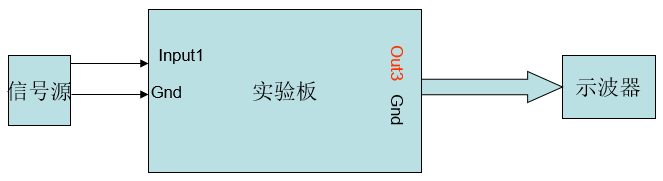
\includegraphics[width = 0.8\linewidth]{dia.png}
	\caption{数字滤波对模拟信号滤波原理图}
	\label{fig:数字滤波对模拟信号滤波原理图}
\end{figure}

IIR滤波器为无限长单位脉冲响应数字滤波器,其传递函数为以下形式:

\begin{align}
	H(z) = \dfrac{\sum\limits_{r = 0}^{m}b_rz^{-r}}
	{1 - \sum\limits_{k = 1}{n}a_kz^{ - k}}
\end{align}

本实验中我们实现一个50阶的IIR滤波器,其低通、高通、带通的频响特性分别如
图\ref{fig:IIR频响特性}所示:

\begin{figure}[htbp]
	\centering
	\begin{subfigure}[htbp]{.45\linewidth}
		\centering
		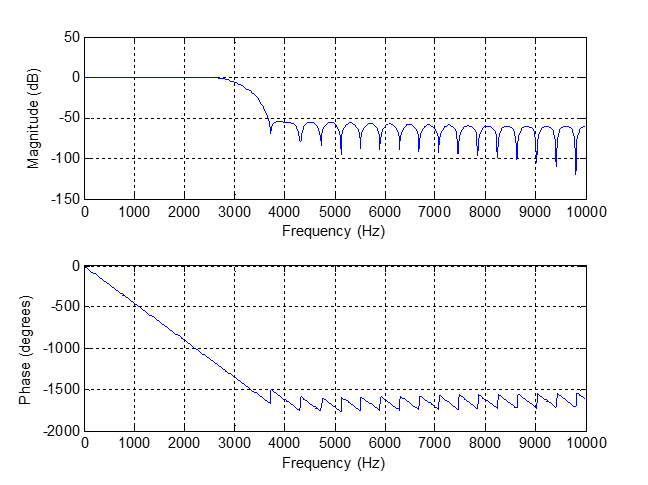
\includegraphics[width = \linewidth]{LP.png}
		\caption{LPIIR}
		\label{fig:LPIIR}
	\end{subfigure}
	\quad
	\begin{subfigure}[htbp]{.45\linewidth}
		\centering
		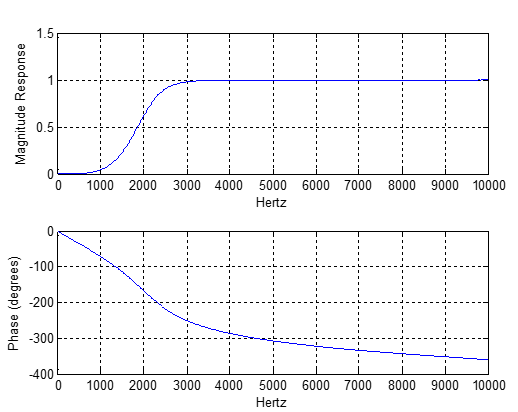
\includegraphics[width = \linewidth]{HP.png}
		\caption{HPIIR}
		\label{fig:HPIIR}
	\end{subfigure}

	\begin{subfigure}[htbp]{.45\linewidth}
		\centering
		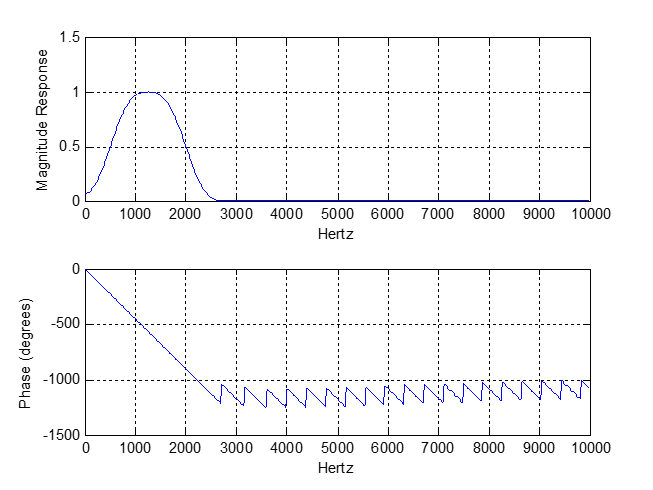
\includegraphics[width = \linewidth]{BP.png}
		\caption{BPIIR}
		\label{fig:BPIIR}
	\end{subfigure}
	\caption{IIR频响特性}
	\label{fig:IIR频响特性}
\end{figure}

本实验中IIR数字滤波器将采用通用的DSP芯片TMS320F2812来实现,其原理图如图
\ref{fig:数字滤波器硬件原理图}所示:

\begin{figure}[htbp]
	\centering
	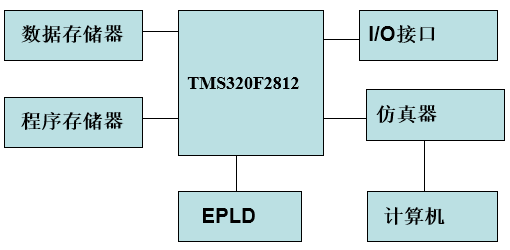
\includegraphics[width = 0.8\linewidth]{hardware.png}
	\caption{数字滤波器硬件原理图}
	\label{fig:数字滤波器硬件原理图}
\end{figure}

TMS320F2812为哈佛结构的32位定点DSP。使用的A/D转换器是ADI公司的12位模数转换器,
D/A转换器为ADI公司的AD768(16位数模转换器)。实验装置包含了A/D、D/A单元和输入滤
波器。

\section{实验仪器、仪表}%
\label{sec:\arabic{chapter}实验仪器、仪表}

\begin{table}[htbp]
	\centering
	\caption{实验仪器、仪表}
	\label{tab:实验仪器、仪表}
	\csvautobooktabular{tab/BOM.csv}
\end{table}

\section{实验预习要求}%
\label{sec:\arabic{chapter}实验预习要求}

认真复习采样定理、IIR滤波器的结构以及A/D 、D/A转换器等有关内容,阅读TMS320F2812的
有关知识及实验原理、实验所用其它器件的性能和使用方法。

\section{实验原理图}%
\label{sec:\arabic{chapter}实验原理图}

\begin{figure}[htbp]
	\centering
	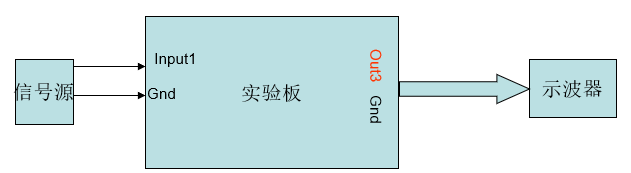
\includegraphics[width = 0.8\linewidth]{scheme.png}
	\caption{实验原理图}
	\label{fig:实验原理图}
\end{figure}

\section{实验内容及步骤}%
\label{sec:\arabic{chapter}实验内容及步骤}

\begin{enumerate}

	\item 按实验连接图检查连线是否正确,然后依次打开信号源、示波器、实验装置
		的电源开关;

	\item 将信号源的频率调至50Hz,$ V_\mathrm{pp}$调至500mV,按试验箱上的提示选择
		1($ f_\mathrm{s} = $20KHz),再选择2(iir),然后选择1(低通:$ \omega_n = $0.3);

	\item 观察示波器上的输出信号。将信号源的频率从50Hz逐渐提高,观察示波器上
		的输出信号幅度的变化规律并作记录(记录点数不得少于10点),记下系统
		的fc ;

	\item 低通数据测量结束后,按6返回,重新选择1($ f_\mathrm{s} = $20KHz),再选择2(iir),然
		后再选择2(高通:$ \omega_n = $0.2);

	\item 重复步骤3的操作,测量高通滤波器的频响特性;

	\item 高通数据测量结束后,按6返回,选择2($ f_\mathrm{s} = $27.9KHz),再选择2(iir) ,然
		后再选择 1(低通:$ \omega_n = $0.3);

	\item 重复步骤3的操作,测量不同采样频率下低通滤波器的频响特性;

	\item 低通数据测量结束后,按6返回,选择2($ f_\mathrm{s} = $27.9KHz),再选择2(iir),然后
		再选择2( 高通:$ \omega_n = $0.2);

	\item 重复步骤3的操作,测量不同采样频率下高通滤波器的频响特性。

\end{enumerate}

\section{实验报告}%
\label{sec:\arabic{chapter}实验报告}

\begin{Exercise}

	写明实验目的、实验原理、实验内容及步骤;

\end{Exercise}

\begin{Answer}

	实验目的见章节\ref{sec:\arabic{chapter}实验目的},实验原理见章节
	\ref{sec:\arabic{chapter}实验原理},实验内容及步骤见章节
	\ref{sec:\arabic{chapter}实验内容及步骤}。

\end{Answer}

\begin{Exercise}

	整理实验数据,在坐标纸上分别画出所测系统的频响特性曲线,比较所测各种滤波器
	带宽与理论带宽的误差;并比较相同$ \omega_n $、不同采样频率下实验所得同种
	滤波器的带宽,得出滤波器带宽与采样频率之间的关系。

\end{Exercise}

\begin{Answer}

	频响特性曲线见图\ref{fig:IIR}。比较图\ref{fig:IIR频响特性}和
	\ref{fig:IIR},可见实验数据与仿真结果比较吻合。数字信号的带宽与采样率成
	正比例关系。

\end{Answer}

\begin{figure}[htbp]
	\centering
	\begin{subfigure}[htbp]{.45\linewidth}
		\centering
		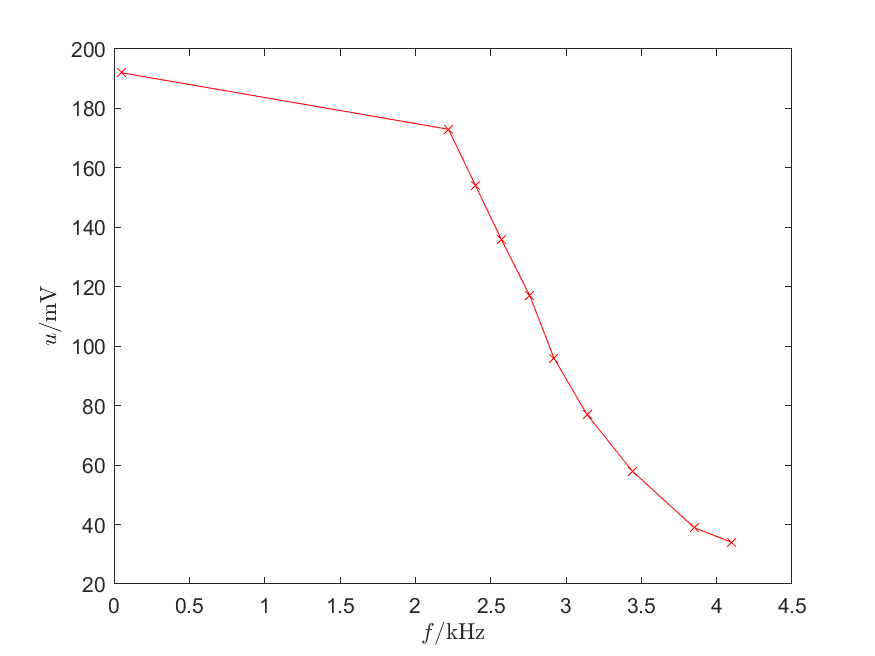
\includegraphics[width = \linewidth]{LPIIR20.png}
		\caption{LPIIR20kHz}
		\label{fig:LPIIR20}
	\end{subfigure}
	\quad
	\begin{subfigure}[htbp]{.45\linewidth}
		\centering
		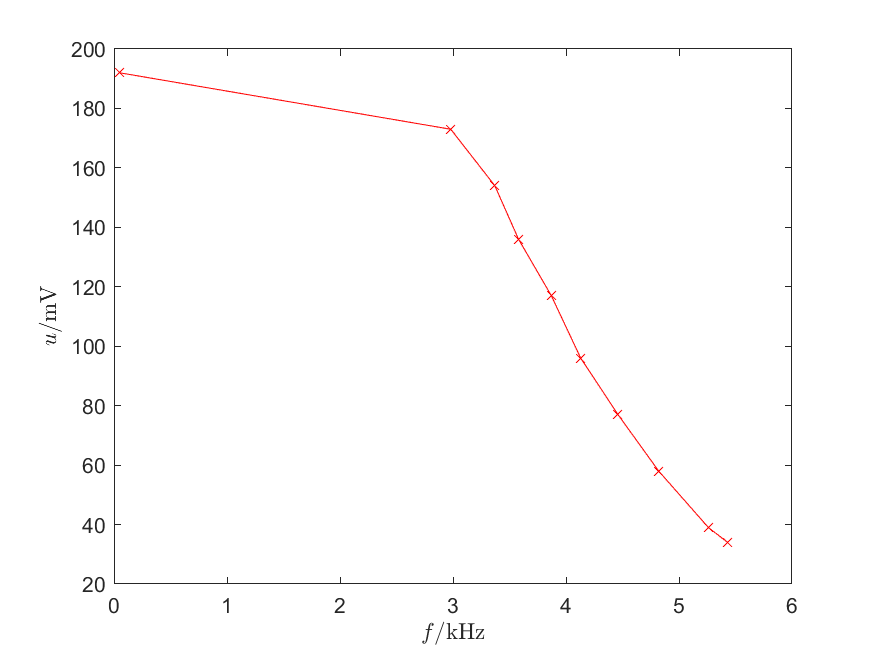
\includegraphics[width = \linewidth]{LPIIR27.png}
		\caption{LPIIR27.9kHz}
		\label{fig:LPIIR27}
	\end{subfigure}

	\begin{subfigure}[htbp]{.45\linewidth}
		\centering
		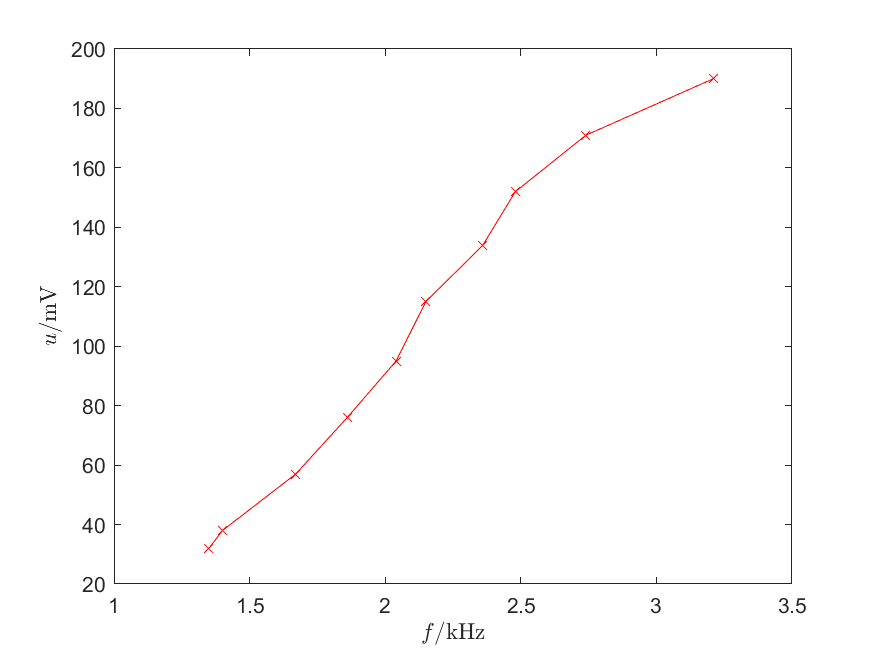
\includegraphics[width = \linewidth]{HPIIR20.png}
		\caption{HPIIR20kHz}
		\label{fig:HPIIR20}
	\end{subfigure}
	\quad
	\begin{subfigure}[htbp]{.45\linewidth}
		\centering
		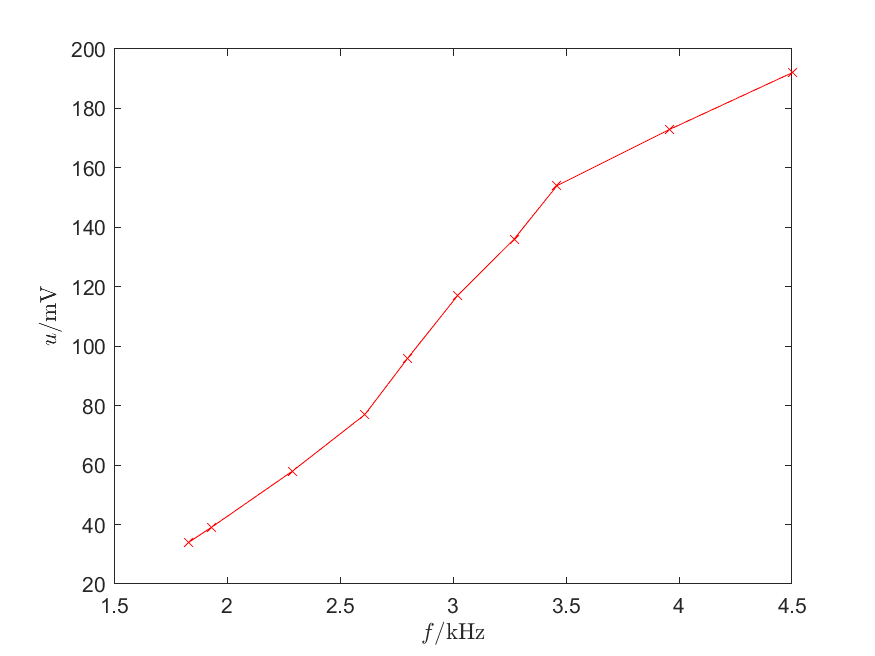
\includegraphics[width = \linewidth]{HPIIR27.png}
		\caption{HPIIR27.9kHz}
		\label{fig:HPIIR27}
	\end{subfigure}
	\caption{IIR}
	\label{fig:IIR}
\end{figure}

\begin{table}[htbp]
	\centering
	\caption{LPIIR20kHz}
	\label{tab:LPIIR20kHz}
	\csvautobooktabular{tab/LPIIR20.csv}
\end{table}

\begin{table}[htbp]
	\centering
	\caption{LPIIR27.9kHz}
	\label{tab:LPIIR27.9kHz}
	\csvautobooktabular{tab/LPIIR27.csv}
\end{table}

\begin{table}[htbp]
	\centering
	\caption{HPIIR20kHz}
	\label{tab:HPIIR20kHz}
	\csvautobooktabular{tab/HPIIR20.csv}
\end{table}

\begin{table}[htbp]
	\centering
	\caption{HPIIR27.9kHz}
	\label{tab:HPIIR27.9kHz}
	\csvautobooktabular{tab/HPIIR27.csv}
\end{table}

\end{document}

